\documentclass[12pt]{article}

\usepackage[margin=1.5in]{geometry}
\usepackage{hyperref}
\usepackage{graphicx}
\hypersetup
{
    colorlinks=true,
    linkcolor=blue,
    filecolor=magenta,      
    urlcolor=blue,
}

\begin{document}
		\begin{titlepage}
		\begin{center}
		
		\huge\bfseries{SOFTWARE DESIGN DOCUMENT}\\
		
	
	    \textsc{\Large SOFTWARE ENGINEERING GROUP 9 PROJECT 5:Tracking Interconnected Twitter Links: Using Graph Database Neo4j }\bigbreak
	    \bigbreak
	    \bigbreak
	    \bigbreak
	    \bigbreak
	    \bigbreak
	    \bigbreak
	    \bigbreak
	      \begin{large}
	    GROUP MEMBERS :\\
     Lindiwe Mncwabe\\
     Clifford Ralikhwatha\\
     Thomas Johannsen\\
	    
	    \end{large}
	    \textsc{\Large DATE : 09/30/2017}\\
	    \end{center}
\end{titlepage}	



\tableofcontents
\listoffigures
\newpage

\bigbreak

\begin{flushleft}
\section{Introduction}
\subsection{Purpose of this Software Design Document}

This software design document describes the architecture,the detailed structure design of Tracking Interconnected Twitter Links: Using Graph Neo4j Database.In practice, requirements and design are inseparable.It is assumed that the reader has read the Specific Requirements Specification document , since this document also defines the implementation details of the
given requirements.
\end{flushleft}


\begin{flushleft}
\subsection{Description of the software}
\bigbreak
The purpose of this software is to graph Twitter data so that hidden trends and
patterns may be revealed.Since this is the first software we are producing, there no other programs to interface
with. With this program you will be able to understand your interaction in the
Twitter world. 
\end{flushleft}

\begin{flushleft}
\subsection{Reference Material}
As sources of information visit:
https://networkdata.ics.uci.edu/resources.php
Learning Neo4j By Rik Van Bruggen
http://network.graphdemos.com/
\end{flushleft}

\bigbreak
\begin{flushleft}
\textbf{1.4Definations,Abbreviations and Acronyms}
\bigbreak

-Neo4j Database :Neo4j is a graph database management system developed by Neo4j, Inc.It is an open-source NoSQL graph database implemented in Java and Scala.\\
-Graph Database :In computing this is a database that uses graph structures for semantic queries with nodes,edges and properties to represent and store data.
-SDLC: Software Development Life Cycle
- UC: use case
- GD: graph database(Neo4j)

\end{flushleft}
\bigbreak
\newpage
\begin{flushleft}

\section{SYSTEM OVERVIEW}

There is enormous information about individuals and how they relate to one another. This information
is useful to individuals, advertisers, politicians and many other organisations.Our software provides means to get links between individuals in social
media.We will be analysing Twitter links using Neo4j database.\\
\bigbreak
\bigbreak
\begin{large}
From the SRS document the Functional user characteristics :
\end{large}\\

- Show all people using twitter\\
- Show all tweets of each person\\
- show retweets, distinguish between followers and non followers\\
- show replies/mentions\\
\bigbreak
\begin{large}
The functional system characteristics of our software describe the system services:\\
\end{large}
-The software returns a list of tweets matching a supplied search item.\\
-The back-end of the project is the management of the Neo4j database.\\
-The front-end is an interface for querying and displaying the results of the graph queries.The user interacts with the representation.\\
-The software is able to handle at least five users without affecting the
user's experience.\\
\end{flushleft}
\begin{flushleft}

\section{SYSTEM ARCHITECTURE}
\bigbreak
The SDD SYSTEM ARCHITECTURE design of the Tracking Interconnected Twitter Links: Using Graph Database Neo4j system contains a detailed description of the software using models.It will attempt to define the functionality of the system, the system's properties and,to a certain extent,provide pseudocodes or ways of explaining the coding process.\\
\bigbreak
\subsection{System Architectural Design}
\bigbreak

\begin{figure}
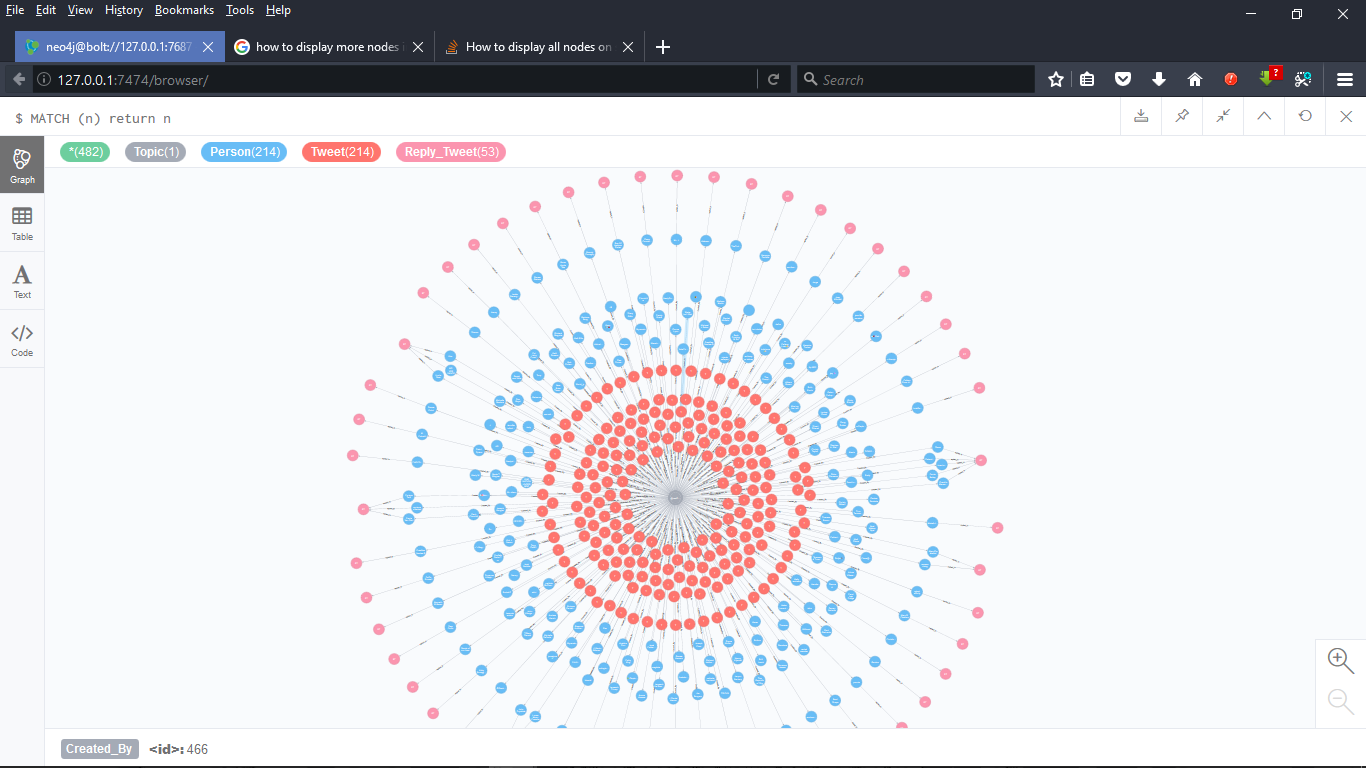
\includegraphics[width=\textwidth]{1}
\caption{Final design} 
\label{fig: 1}
An overview of the nodes and connections in the database, differentiated by colour
\end{figure}

\begin{figure}
\includegraphics[width=6cm]{Flow}\newline
\caption{Data process} 
\label{fig: 2}
Graphic overview of the path data takes from real world input to real world output, and the programs used at each step.
\end{figure}

\begin{figure}
\includegraphics[width=6cm]{Graph}\newline
\caption{Neo4j database} 
\label{fig: 3}
The initial design of the database. All listed properties and some more will be captured by the node, no properties saved in edges as of this design.
\end{figure}

\newpage
\bigbreak
\bigbreak
\section{DATA DESIGN}
\subsection{Database design(Neo4j)}

As a native graph database, Neo4j is specifically optimized to store and traverse these (twitter) graphs of connected data.
People and tweets can easily be represented as nodes, and allow for a good overview as well as a logical structure to how linked different people are in an age of instant global communication.
\newline
With a central node representing the search phrase for a topic to filter the tweets by, and people and tweet nodes branching out from it, we get something similar to Figure 1. These nodes will store a lot of information such as date, age, gender, topic. This allows different graphs to be made when filtering by these properties. 
We could include a person's followers, however many have 1000+ friends/followers, which uses up graph space unless filtered by relevance somehow.

Location would be a nice property to include, however some people chose not to chase their location with twitter, and those that do have very different results based on their providers. From the test data 3 locations we had were: "\#gameofthrones", "Kenya" and "Basin, WY, United States". 3 very different results. In order for location to always be useful it would have to be analysed and sorted, probably through an external tool. We will include it as a location, but not use it further, it can be used as a search filter.

\section{USER INTERFACE DESIGN}

The User Interface is a crucial aspect of the system.The Neo4j browser offers easy to use manipulation tools and a nice graphic visualisation, it's the best choice among many similar tools due the compatibility with the Neo4j database.
\subsection{Overview of User Interface}

\begin{figure}
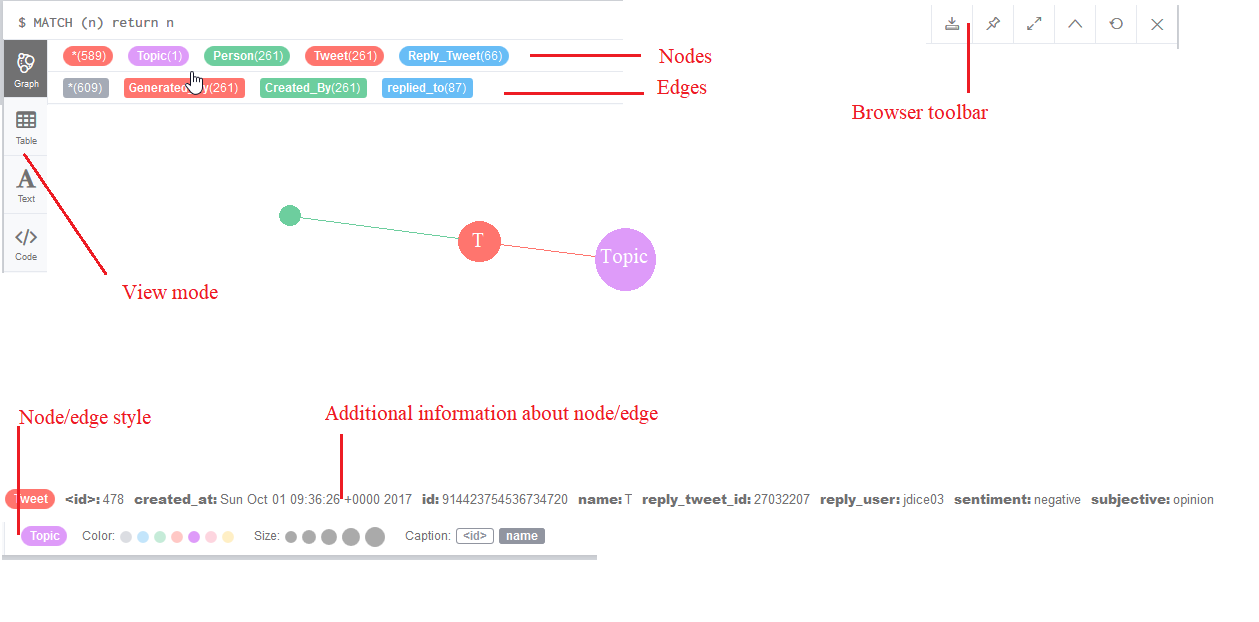
\includegraphics[width=\textwidth]{User}
\caption{Browser interface} 
\label{fig: 4}
An overview of the nodes and connections in the database, differentiated by colour. Properties of nodes can be seen by clicking on a node. Node/edge style can be modifies by selecting the type of node/edge at the top of the graph and then styling them at the bottom.\newline
View mode offers different ways to see the data, or code, "Table" and "text" show more text heavy versions of databases while "code" shows how the code runs to return results for a query. All view modes offer the same information, it comes down to personal preference which is preferred as certain data is more apparent in different view modes.\newline
"Match(n) return n" returns all nodes in the database(max 300 default), various other Cypher commands can be entered into the command line to run a query on the data. Some of these commands can be found in the Cipher Queries document. Ideally if this were hosted on a server these commands would be replaced with an overlay that automates the queries for a simpler user interface. 
\end{figure}
\newpage
\section{SOFTWARE APPLICATION}

Our software uses Neo4j database. Social media networks are already graphs, using Neo4j improves the quality and the speed of development for social media application (such as twitter) by reducing the time you spend data modeling.A tool like this has many applications, certain tweet patterns could signal to an account being bot operated, it can be used to find out what a certain age, race, gender, location are tweeting about a certain topic. The first application that pops to mind is targeted advertising, but many more exist. This is also a great tool for companies to see how a target market, or group of people react to their product or incentives. 

\newpage
\section{ BIBLIOGRAPHY}
\textbf{[1]Vliet, Hans Van, “Software Engineering Principles and Practice”, 2001, Wiley}\\
\textbf{[2]“IEEE Standard for Distributed Interactive Simulation – Application Protocols”, 1995}\\
\textbf{[3]Software Engineering,10th Edition,published by Pearson,2015,ISBN-13:978-0133943030}






\end{flushleft}


\end{document}